\documentclass[border=6pt]{standalone}
\usepackage{amsmath}
\usepackage{amssymb}
\usepackage{tikz}
\usepackage{pgfplots}
\pgfplotsset{compat=1.18}
\usetikzlibrary{arrows.meta,calc,positioning}
\begin{document}
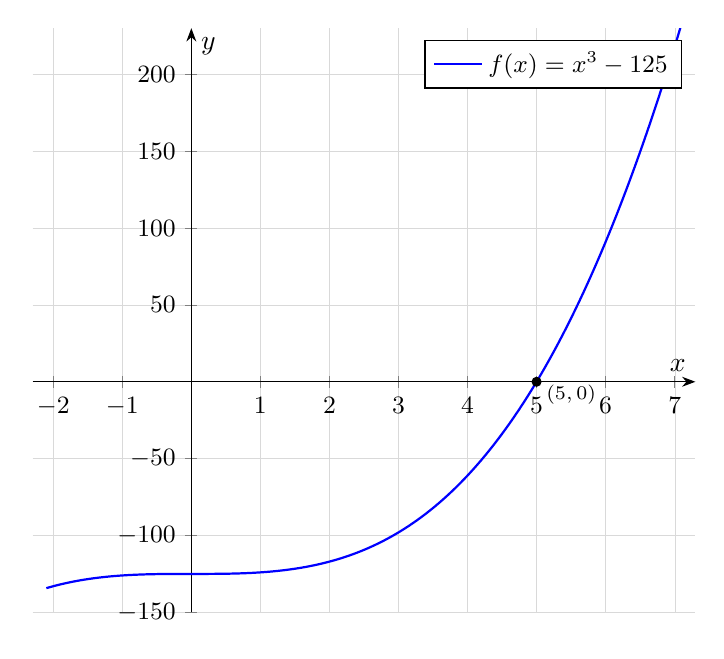
\begin{tikzpicture}
\begin{axis}[
    axis lines = middle,
    xlabel = {$x$}, ylabel = {$y$},
    grid=both,
    grid style={line width=.1pt, draw=gray!30},
    axis line style={-Stealth},
    legend style={font=\small},
    tick label style={font=\small},
    xmin=-2.3, xmax=7.3, ymin=-150, ymax=230,
    xtick={-2,-1,0,1,2,3,4,5,6,7},
    ytick={-150,-100,-50,0,50,100,150,200},
    width=10cm, height=9cm,
]
\addplot[domain=-2.1:7.1, samples=150, thick, blue] {x^3-125};
\addlegendentry{$f(x)=x^3-125$}
\addplot[only marks, mark=*, mark size=1.6pt, black] coordinates {(5,0)};
\node[anchor=north west, font=\scriptsize] at (axis cs:5,4) {$(5,0)$};
\end{axis}
\end{tikzpicture}
\end{document}
